%% Le lingue utilizzate, che verranno passate come opzioni al pacchetto babel. Come sempre, l'ultima indicata sarà quella primaria.
%% Se si utilizzano una o più lingue diverse da "italian" o "english", leggere le istruzioni in fondo.
\def\thudbabelopt{english,italian}
%% Valori ammessi per target: bach (tesi triennale), mst (tesi magistrale), phd (tesi di dottorato).
%% Valori ammessi per aauheader: '' (vuoto -> nessun header Alpen Adria Univeristat), aics (Department of Artificial Intelligence and Cybersecurity), informatics (Department of Informatics Systems). Il nome del dipartimento è allineato con la versione inglese del logo UniUD.
%% Valori ammessi per style: '' (vuoto -> stile moderno), old (stile tradizionale).
\documentclass[target=bach,aauheader=,style=]{thud}

%% --- Informazioni sulla tesi ---
%% Per tutti i tipi di tesi
% Scommentare quello di interesse, o mettete quello che vi pare
\course{Informatica}
%\course{Internet of Things, Big Data e Web}
%\course{Matematica}
%\course{Comunicazione Multimediale e Tecnologie dell'Informazione}
\title{Un sistema distribuito per l'analisi della topologia di reti di calcolatori}
\author{Diego Cirillo}
\supervisor{Prof.\ Marino Miculan}
\cosupervisor{Dott.\ Matteo Paier}
%\tutor{Guido Necchi}
%% Campi obbligatori: \title, \author e \course.
%% Altri campi disponibili: \reviewer, \tutor, \chair, \date (anno accademico, calcolato in automatico), \rights
%% Con \supervisor, \cosupervisor, \reviewer e \tutor si possono indicare più nomi separati da \and.
%% Per le sole tesi di dottorato:
%\phdnumber{313}
%\cycle{XXVIII}
%\contacts{Via della Sintassi Astratta, 0/1\\65536 Gigatera --- Italia\\+39 0123 456789\\\texttt{http://www.example.com}\\\texttt{inbox@example.com}}

%% --- Pacchetti consigliati ---
%% pdfx: per generare il PDF/A per l'archiviazione. Necessario solo per la versione finale
\usepackage[a-1b]{pdfx}
%% hyperref: Regola le impostazioni della creazione del PDF... più tante altre cose. Ricordarsi di usare l'opzione pdfa.
\usepackage[pdfa]{hyperref}
%% tocbibind: Inserisce nell'indice anche la lista delle figure, la bibliografia, ecc.
\graphicspath{ {./images/} }
%% --- Stili di pagina disponibili (comando \pagestyle) ---
%% sfbig (predefinito): Apertura delle parti e dei capitoli col numero grande; titoli delle parti e dei capitoli e intestazioni di pagina in sans serif.
%% big: Come "sfbig", solo serif.
%% plain: Apertura delle parti e dei capitoli tradizionali di LaTeX; intestazioni di pagina come "big".
\usepackage{placeins}

\begin{document}
\maketitle

%% Dedica (opzionale)
%\begin{dedication}
%	Al mio cane,\par per avermi ascoltato mentre ripassavo le lezioni.
%\end{dedication}

%% Ringraziamenti (opzionali)
%\acknowledgements
%Sed vel lorem a arcu faucibus aliquet eu semper tortor. Aliquam dolor lacus, semper vitae ligula sed, blandit iaculis leo. Nam pharetra lobortis leo nec auctor. Pellentesque habitant morbi tristique senectus et netus et malesuada fames ac turpis egestas. Fusce ac risus pulvinar, congue eros non, interdum metus. Mauris tincidunt neque et aliquam imperdiet. Aenean ac tellus id nibh pellentesque pulvinar ut eu lacus. Proin tempor facilisis tortor, et hendrerit purus commodo laoreet. Quisque sed augue id ligula consectetur adipiscing. Vestibulum libero metus, lacinia ac vestibulum eu, varius non arcu. Nam et gravida velit.

%% Sommario (opzionale)
%\abstract
%La crescente complessità delle reti di calcolatori moderne richiede strumenti sofisticati per la loro analisi e gestione. Questa tesi presenta la progettazione e lo sviluppo di un sistema distribuito innovativo, capace di esplorare e mappare in modo efficiente le topologie di reti di grandi dimensioni. Il sistema proposto è in grado di estrarre informazioni significative sulla struttura della rete, identificando pattern, anomalie e potenziali vulnerabilità. L'obiettivo finale è fornire ai network administratori un quadro completo e dettagliato della loro infrastruttura, supportando decisioni informate e ottimizzando le performance della rete.

%% Indice
\tableofcontents

%% Lista delle tabelle (se presenti)
%\listoftables

%% Lista delle figure (se presenti)
\listoffigures
!TODO

%% Corpo principale del documento
\mainmatter

%% Parte
%% La suddivisione in parti è opzionale; solitamente sono sufficienti i capitoli.
%\part{Parte}

%% Capitolo
\chapter{Introduzione}
\section{Motivazioni dello Studio}
\subsection{Importanza dell'analisi della topologia di rete.}
L'analisi della topologia di rete è un'attività cruciale per la gestione, la sicurezza e l'ottimizzazione delle infrastrutture di rete. La topologia di rete rappresenta la struttura fisica e logica di una rete, delineando come i dispositivi (come router, switch, server, ecc.) siano interconnessi e come i dati fluiscano tra di essi. Una comprensione dettagliata della topologia è essenziale per diverse ragioni:
\begin{itemize}
  \item Ottimizzazione delle Prestazioni: Una corretta analisi della topologia consente di identificare colli di bottiglia, percorsi inefficienti e configurazioni subottimali che possono influenzare negativamente le prestazioni della rete. Migliorando la topologia, si possono ottenere connessioni più rapide e una distribuzione del traffico più bilanciata.
  \item Gestione e Manutenzione: Conoscere la topologia della rete permette agli amministratori di pianificare meglio le operazioni di manutenzione, minimizzando i tempi di inattività e assicurando la continuità dei servizi. Inoltre, facilita la gestione delle risorse di rete, come l'allocazione degli indirizzi IP e la configurazione dei dispositivi.
  \item Sicurezza: L'analisi della topologia di rete è fondamentale per la sicurezza. Permette di identificare punti deboli nella struttura della rete, come collegamenti non protetti o dispositivi non autorizzati. Questo consente di implementare misure di sicurezza più efficaci, come firewall e segmentazioni di rete.
  \item Rilevamento e Risoluzione dei Problemi: In caso di problemi di rete, una mappa precisa della topologia aiuta a individuare rapidamente la causa dei malfunzionamenti, facilitando una risoluzione tempestiva e riducendo i tempi di inattività.
  \item Scalabilità: Una buona comprensione della topologia è essenziale quando si vuole espandere la rete. Aiuta a garantire che l'espansione avvenga in modo efficiente, senza compromettere le prestazioni o la sicurezza della rete.
\end{itemize}

\subsection{Scopi e obiettivi della tesi.}
La tesi ha come scopo principale la progettazione e lo sviluppo di un sistema distribuito innovativo per l'analisi della topologia di reti di calcolatori, che superi i limiti degli strumenti attualmente disponibili, come SNMP (Simple Network Management Protocol) e altri metodi tradizionali.
\newline
Obiettivi Specifici:
\begin{itemize}
  \item Identificazione delle Limitazioni degli Strumenti Esistenti:
    \begin{itemize}
      \item Analizzare i principali strumenti attualmente utilizzati per l'analisi della topologia di rete, evidenziando le loro carenze in termini di accuratezza, scalabilità, efficienza e sicurezza.
    \item Evidenziare in particolare i limiti di SNMP, come la sua dipendenza da dati statici, la mancanza di supporto per reti complesse e l'inefficienza nella gestione di grandi volumi di dati in tempo reale.
    \end{itemize}

  \item Progettazione di un'Architettura Distribuita:
    \begin{itemize}
      \item Sviluppare un'architettura di sistema distribuita che permetta un'analisi più accurata e dinamica della topologia di rete.
      \item Garantire che il sistema sia scalabile e in grado di gestire grandi reti eterogenee, mantenendo un basso impatto sulle risorse di rete.
    \end{itemize}
    
  %\item Sviluppo di Algoritmi Innovativi:
  %  \begin{itemize}
  %    \item Progettare e implementare algoritmi avanzati per il rilevamento e l'analisi della topologia, che siano in grado di adattarsi dinamicamente ai cambiamenti della rete.
  %    \item Migliorare l'efficienza del sistema, riducendo la latenza e ottimizzando l'uso delle risorse.
  %  \end{itemize}

  %\item Valutazione delle Prestazioni:
  %  \begin{itemize}
  %    \item Confrontare le prestazioni del sistema proposto con quelle degli strumenti esistenti, utilizzando criteri come accuratezza della mappatura, tempo di risposta, utilizzo delle risorse e sicurezza.
  %    \item Testare il sistema in diversi scenari reali per valutarne l'efficacia e identificare eventuali aree di miglioramento.
  %  \end{itemize}


  \item Contributo alla Comunità Scientifica e Industriale:
    \begin{itemize}
      \item Fornire una soluzione innovativa che possa essere utilizzata in ambito accademico e industriale per migliorare la gestione e la sicurezza delle reti di calcolatori.
      \item Contribuire alla letteratura esistente con nuove metodologie e strumenti per l'analisi della topologia di rete.
    \end{itemize}

\end{itemize}



\section{Struttura della Tesi}
\subsection{Breve panoramica dei capitoli successivi.}
Questa tesi è organizzata in x(!TODO) capitoli, ciascuno dei quali affronta aspetti fondamentali dello sviluppo e dell'analisi di un sistema distribuito per l'analisi della topologia di reti di calcolatori. Di seguito viene presentata una panoramica della struttura della tesi.

\begin{itemize}
  \item Capitolo 1: Introduzione
  \begin{itemize}
    \item[] Questo capitolo introduce il tema centrale della tesi, evidenziando l'importanza dell'analisi della topologia di rete. Vengono inoltre delineati gli scopi e gli obiettivi del lavoro, insieme alla struttura generale della tesi.
  \end{itemize}

  \item Capitolo 2: Stato dell'Arte
    \begin{itemize}
      \item[] Nel secondo capitolo vengono esaminati i concetti fondamentali di topologia di rete e vengono descritti i metodi comuni utilizzati per la sua analisi. Viene inoltre condotta un'analisi critica degli strumenti attualmente disponibili, con particolare attenzione ai loro limiti e alle carenze, soprattutto riguardo a SNMP.
    \end{itemize}


  %\item Capitolo 3: Problemi Identificati
  %  \begin{itemize}
  %    \item In questo capitolo vengono discussi in dettaglio i problemi principali che emergono dall'utilizzo degli strumenti esistenti per l'analisi della topologia di rete. Vengono identificati e descritti i limiti in termini di accuratezza, scalabilità, latenza, efficienza, sicurezza e privacy.
  %  \end{itemize}


  \item    Capitolo 3: Requisiti per un Nuovo Sistema
    \begin{itemize}
      \item[] Questo capitolo delinea gli obiettivi e i requisiti di un sistema distribuito innovativo, progettato per superare i limiti degli strumenti esistenti. Viene presentata un'architettura distribuita proposta, insieme ai meccanismi e alle strategie necessari per un'efficace raccolta e analisi dei dati di rete.
    \end{itemize}

  \item Capitolo 4: Progettazione del Sistema Proposto
    \begin{itemize}
      \item[] Il quarto capitolo descrive in dettaglio l'architettura del sistema proposto, i protocolli di comunicazione utilizzati, gli algoritmi sviluppati per l'analisi della topologia e le misure di sicurezza adottate. Viene fornita una descrizione tecnica della progettazione del sistema, enfatizzando le soluzioni innovative implementate.
    \end{itemize}

  \item Capitolo 5: Implementazione
    \begin{itemize}
      \item[] In questo capitolo viene descritta l'implementazione pratica del sistema proposto. Viene esaminata la scelta delle tecnologie utilizzate, il processo di sviluppo del prototipo e i test effettuati per validare il sistema. Sono inoltre inclusi dettagli sull'integrazione delle diverse componenti.
    \end{itemize}

  \item Capitolo 6: Valutazione delle Prestazioni
    \begin{itemize}
      \item[] Il sesto capitolo presenta una valutazione delle prestazioni del sistema sviluppato, confrontandolo con gli strumenti esistenti. Vengono analizzati i risultati dei test effettuati in vari scenari, evidenziando i punti di forza e le possibili aree di miglioramento del sistema proposto.
    \end{itemize}

  \item Capitolo 7: Conclusioni e Lavori Futuri
    \begin{itemize}
      \item[] L'ultimo capitolo riassume i principali risultati ottenuti nel corso della tesi, riflettendo sui limiti della soluzione proposta e suggerendo direzioni future per la ricerca e lo sviluppo in questo campo.
    \end{itemize}

\end{itemize}


\chapter{Stato dell'Arte}
\label{art}
\section{Analisi della Topologia di Rete}
\subsection{Metodi comuni di analisi della topologia.}
L'analisi della topologia di rete implica l'identificazione, la mappatura e la valutazione della struttura della rete, al fine di ottimizzarne il funzionamento e la gestione. Ecco i metodi più comuni utilizzati per questa analisi:
\subsubsection{SNMP (Simple Network Management Protocol):}
    \begin{itemize}
      \item Descrizione: SNMP è un protocollo standardizzato per la gestione e il monitoraggio dei dispositivi di rete. Utilizzato per raccogliere informazioni sulla configurazione e lo stato dei dispositivi di rete, come router e switch.
      \item Vantaggi: Facilità d'uso, ampiamente supportato dai dispositivi di rete, consente di monitorare e gestire una vasta gamma di informazioni.
      \item Svantaggi: Limitato nella capacità di rilevare dinamicamente i cambiamenti nella topologia, difficoltà nell'analizzare reti complesse o eterogenee, problemi di scalabilità.
    \end{itemize}

\subsubsection{Traceroute:}
    \begin{itemize}
      \item Descrizione: Traceroute è uno strumento diagnostico che mostra il percorso che i pacchetti di dati seguono attraverso una rete IP verso una destinazione specifica, identificando tutti i router attraversati.
      \item Vantaggi: Utile per diagnosticare problemi di rete e identificare i percorsi dei dati tra dispositivi.
      \item Svantaggi: Limitato alle reti IP, non fornisce una visione completa della topologia, può essere bloccato da firewall o altri dispositivi di sicurezza.
    \end{itemize}

\subsubsection{NetFlow/IPFIX:}
    \begin{itemize}
      \item Descrizione: NetFlow (e la sua evoluzione IPFIX) è un protocollo sviluppato da Cisco per raccogliere informazioni sui flussi di dati che attraversano un router o uno switch. Fornisce dettagli sulle conversazioni di rete tra dispositivi.
      \item Vantaggi: Permette di monitorare il traffico di rete in dettaglio, utile per analisi del traffico e rilevamento di anomalie.
      \item Svantaggi: Non fornisce direttamente una mappa della topologia, ma piuttosto informazioni sui flussi di traffico, richiede una notevole capacità di elaborazione e archiviazione dei dati.
    \end{itemize}

\subsubsection{LLDP (Link Layer Discovery Protocol):}
    \begin{itemize}
      \item Descrizione: LLDP è un protocollo di livello datalink utilizzato per scoprire dispositivi vicini e condividere informazioni sulla loro configurazione.
      \item Vantaggi: Consente la scoperta automatica dei dispositivi connessi alla rete e facilita la gestione della rete.
      \item Svantaggi: Limitato al livello 2 (livello di collegamento dati) della pila OSI, quindi non fornisce una visione completa della topologia a livello IP o superiore.
    \end{itemize}

\noindent Questi metodi offrono diverse prospettive sull'analisi della topologia di rete, ognuno con i propri punti di forza e debolezze. Tuttavia, nessuno di essi, preso singolarmente, offre una soluzione completa per l'analisi della topologia di reti complesse e dinamiche, evidenziando la necessità di strumenti più avanzati e integrati.

\subsection{Problemi dell'utilizzo di SNMP per l'Analisi della Topologia}
SNMP (Simple Network Management Protocol) è uno dei protocolli più utilizzati per il monitoraggio e la gestione delle reti, ma presenta diversi limiti significativi quando viene utilizzato per l'analisi della topologia di rete. Di seguito vengono analizzati i principali problemi associati all'uso di SNMP in questo contesto.
\begin{itemize}

  \item Scalabilità Limitata
    \begin{itemize}
      \item Overhead di Polling: SNMP si basa su un meccanismo di polling, in cui un sistema di gestione della rete (NMS) invia richieste ai dispositivi per ottenere informazioni sul loro stato. In una rete di grandi dimensioni, il numero di richieste necessarie per raccogliere i dati da tutti i dispositivi può diventare ingente, causando un significativo overhead di rete e aumentando il carico sui dispositivi stessi.
      \item Crescita Esponenziale del Traffico di Gestione: Man mano che il numero di dispositivi in rete aumenta, anche il volume del traffico di gestione generato da SNMP cresce esponenzialmente, rischiando di congestionare la rete e rallentare le operazioni di monitoraggio.
    \end{itemize}

  \item Visione Statica della Topologia
  \begin{itemize}
      \item Informazioni Non in Tempo Reale: Poiché SNMP si basa su un ciclo di polling, i dati raccolti rappresentano istantanee dello stato della rete in momenti specifici. Questo significa che i cambiamenti dinamici nella topologia, come l'aggiunta o la rimozione di dispositivi, potrebbero non essere rilevati immediatamente, portando a una rappresentazione obsoleta della rete.
      \item Mancanza di Rilevamento dei Cambiamenti Dinamici: In reti moderne, dove la topologia può cambiare rapidamente a causa della virtualizzazione, del cloud computing o delle configurazioni dinamiche, SNMP non riesce a rilevare e adattarsi efficacemente a questi cambiamenti.
  \end{itemize}


  \item Sicurezza Limitata
    \begin{itemize}
      \item Vulnerabilità di SNMPv1 e SNMPv2: Le prime versioni di SNMP (v1 e v2) non supportano meccanismi di sicurezza robusti, come l'autenticazione o la crittografia. Le informazioni vengono trasmesse in chiaro, rendendo la rete vulnerabile a intercettazioni e attacchi man-in-the-middle.
      \item Complessità di SNMPv3: Sebbene SNMPv3 introduca miglioramenti significativi in termini di sicurezza, includendo l'autenticazione e la crittografia, la sua implementazione è complessa e richiede una configurazione accurata per essere efficace. La complessità può scoraggiare la piena adozione o portare a configurazioni non sicure.
    \end{itemize}

  \item Complessità di Configurazione e Manutenzione
    \begin{itemize}
      \item Configurazione Manuale: Per ottenere una visione accurata della topologia, ogni dispositivo deve essere configurato per rispondere alle richieste SNMP, e questa configurazione deve essere mantenuta e aggiornata nel tempo. In grandi reti, questo può diventare un compito oneroso.
      \item Varianza di Supporto tra Vendor: Non tutti i dispositivi di rete supportano SNMP nello stesso modo, e le implementazioni possono variare tra i diversi vendor, portando a problemi di interoperabilità e difficoltà nel mantenere una mappa coerente della rete.
    \end{itemize}

  \item Limitata Capacità di Mappatura della Topologia
    \begin{itemize}
      \item Dati Limitati sulla Connettività: SNMP è utile per raccogliere dati su singoli dispositivi, come lo stato delle interfacce, l'uso della CPU o della memoria, ma non fornisce informazioni dettagliate sulle connessioni tra i dispositivi. Questo rende difficile ottenere una mappa completa e accurata della topologia della rete.
      \item Assenza di Informazioni di Layer 2: SNMP è principalmente focalizzato sui dati di Layer 3 (IP), mancando spesso le informazioni di Layer 2 (Ethernet), che sono cruciali per una mappatura dettagliata della topologia di rete, specialmente in ambienti complessi con VLAN e altri segmenti logici.
    \end{itemize}


  \item Problemi di Performance
    \begin{itemize}
      \item Impatto sulle Risorse del Dispositivo: L'elaborazione delle richieste SNMP può consumare risorse significative del dispositivo, specialmente su dispositivi con capacità hardware limitate. Questo può degradare le prestazioni del dispositivo stesso, influenzando la qualità del servizio di rete.
      \item Ritardi nella Raccolta dei Dati: In reti con molti dispositivi o con un utilizzo intensivo di SNMP, i ritardi nella raccolta e nell'analisi dei dati possono aumentare, rendendo meno tempestive le informazioni disponibili e, di conseguenza, meno utile l'analisi della topologia.
    \end{itemize}
\end{itemize}


\chapter{Soluzione proposta}
Il sistema che propongo per l'analisi della topologia di rete è basato su un'architettura distribuita che sfrutta un insieme di probes (sonde) per scansionare contemporaneamente diverse sezioni della rete. Ogni probe utilizza Nmap per raccogliere informazioni dettagliate, che vengono poi aggregate in un database centralizzato. Questo approccio consente di ottenere una visione completa e accurata della topologia di rete, superando i limiti di scalabilità e accuratezza degli strumenti tradizionali.

Nell'architettura proposta, le probes sono distribuite strategicamente all'interno della rete, con ciascuna di esse responsabile di una specifica area. Operando simultaneamente, le probes eseguono scansioni parallele, raccogliendo dati sui dispositivi di rete, sulle connessioni e sui servizi attivi. I dati raccolti vengono inviati a un database centralizzato, dove vengono normalizzati e aggregati per creare una mappa coerente e dettagliata della rete. L'architettura include anche un sistema di visualizzazione interattivo che permette agli amministratori di esplorare la topologia in tempo reale, monitorando le modifiche e aggiornando continuamente le informazioni.

Uno dei principali vantaggi di questo sistema è la sua scalabilità. A differenza degli approcci centralizzati, che possono soffrire di colli di bottiglia man mano che la rete cresce, l'uso di probes distribuite consente di gestire efficacemente anche le reti più estese. L'elaborazione parallela delle scansioni riduce il tempo necessario per mappare l'intera rete, distribuendo il carico di lavoro e prevenendo sovraccarichi sui singoli dispositivi.

Un altro vantaggio significativo riguarda l'accuratezza dei dati raccolti. Poiché ogni probe ha una visione dettagliata della porzione di rete che le è assegnata, il sistema garantisce una copertura completa e precisa della topologia. Inoltre, il processo di aggregazione centralizzato consente di risolvere eventuali discrepanze nei dati e di eliminare le ridondanze, fornendo una rappresentazione accurata e aggiornata della rete.

L'architettura proposta offre anche maggiore resilienza rispetto ai sistemi tradizionali. Se una o più probes dovessero fallire, il sistema può continuare a funzionare con le probes rimanenti, garantendo la continuità operativa. Inoltre, il sistema è altamente flessibile: può essere facilmente adattato per includere nuove probes o per modificare l'area di scansione di quelle esistenti, rendendolo capace di rispondere rapidamente ai cambiamenti nella rete.

Dal punto di vista della sicurezza, il sistema è progettato per ridurre al minimo l'esposizione a potenziali attacchi. I dati raccolti vengono trasmessi al database centrale utilizzando canali sicuri e crittografati, proteggendo le informazioni sensibili da eventuali intercettazioni.

In sintesi, l'architettura distribuita proposta rappresenta un significativo miglioramento rispetto agli strumenti tradizionali di analisi della topologia di rete. Essa combina scalabilità, accuratezza, resilienza e sicurezza, offrendo una soluzione completa per la mappatura e il monitoraggio delle reti moderne.

\chapter{Progettazione del Sistema}
\section{Architettura del Sistema}
\subsection{Descrizione dettagliata dell'architettura distribuita}
Il sistema è composto da una architettura client-server nella quale il backend si occupa di fare le scansioni, di salvarne i risultati e di fornirli al frontend dove possono essere visualizzati dagli utenti dovrebbero interagire solo con esso. 


\begin{figure}[h]
  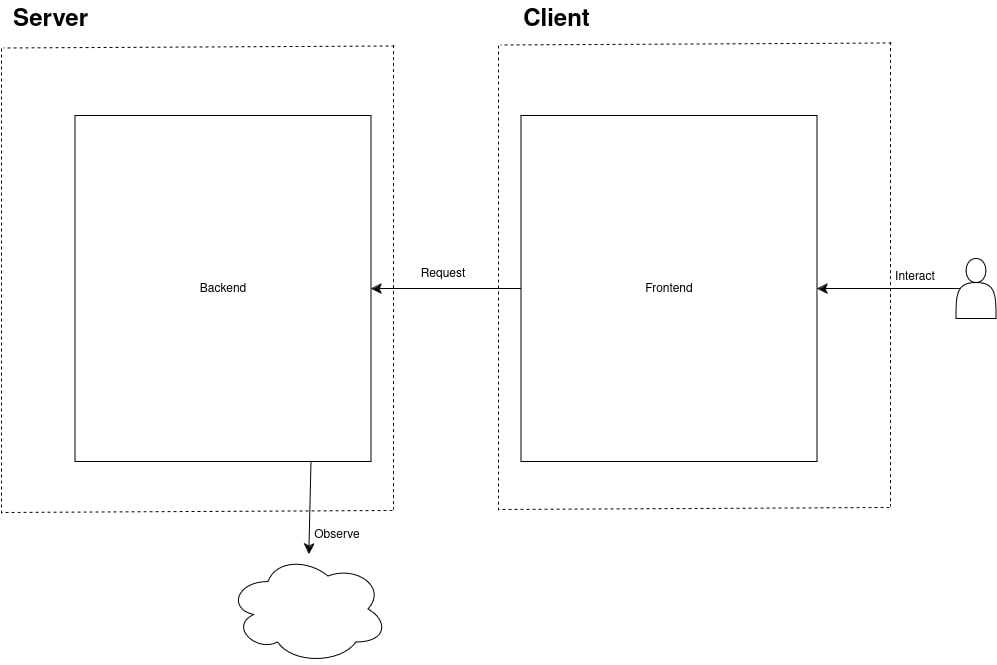
\includegraphics[width=15cm, height=10cm]{client_server}
  \centering
\end{figure}

\FloatBarrier

Per organizzazione e scalabilità abbiamo diviso l'architettura in 6 moduli principali.


\begin{figure}[h]
  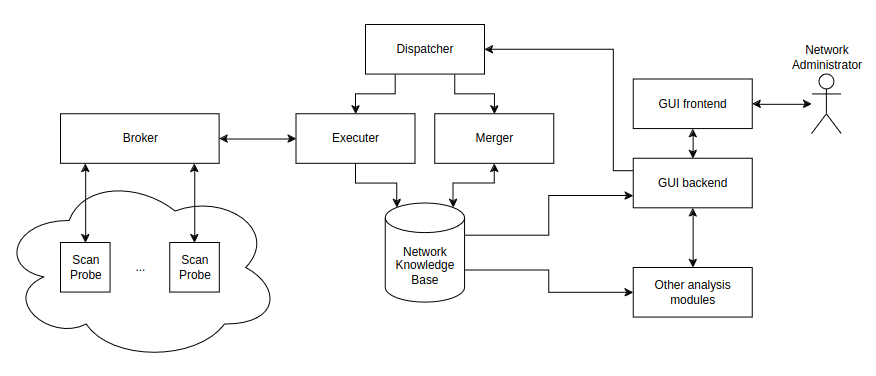
\includegraphics[width=15cm, height=10cm]{moduli_new}
  \centering
\end{figure}

\FloatBarrier

\subsubsection{Scan Probes}
Gli Scan Probes sono moduli che vengono collocati in giro per la rete a raccogliere informazioni. 
Ricevuto un comando il probe lo interpreta, esegue l'opportuna scansione e deserializza l'output dello scan.


\begin{figure}[h]
  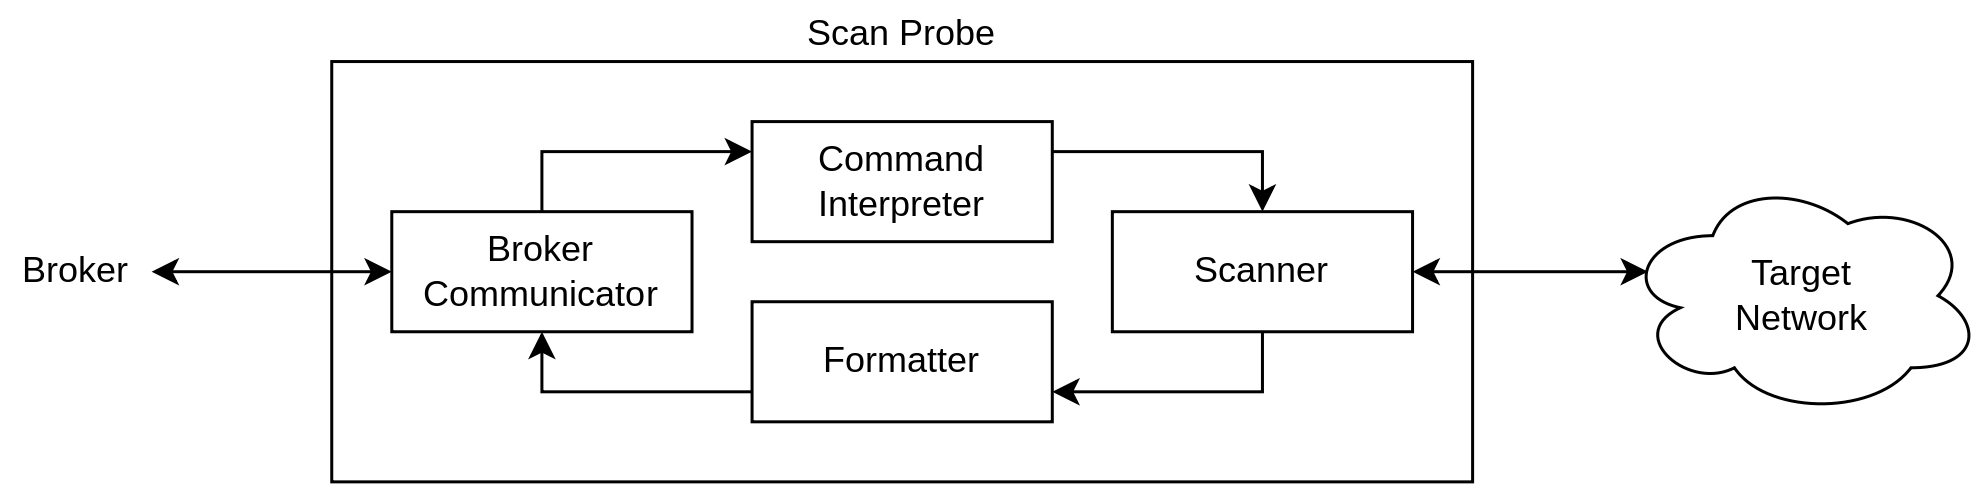
\includegraphics[width=14cm, height=8cm]{probe}
  \centering
\end{figure}
\FloatBarrier


\subsubsection{Dispatcher} 
Il Dispatcher è il modulo che controlla e coordina le operazioni necessarie per le esecuzioni delle scansioni.
Riceve un comando dal Frontend che viene interpretato e mandato allo Scheduler che interagisce con l'Executer ed il Merger per eseguire la scansione e salvarla.

\begin{figure}[h]
  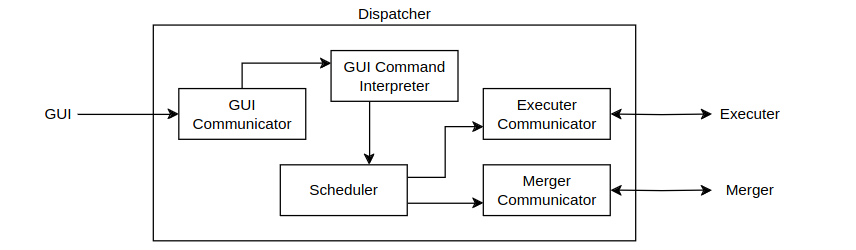
\includegraphics[width=14cm, height=8cm]{dispatcher}
  \centering
\end{figure}

\FloatBarrier

\subsubsection{Executer} 
L'Executer riceve un comando dallo Scheduler e coordina gli Scan Probes nell'esecuzione della scansione tramite un broker di messaggi idoneo. I risultati delle scansioni vengono poi salvati nel Network Knowledge Base.

\begin{figure}[h]
  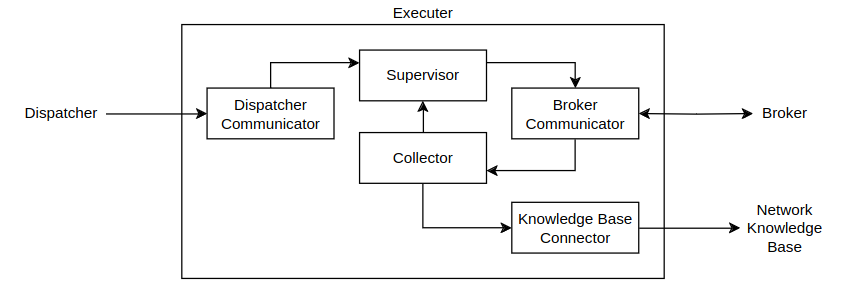
\includegraphics[width=14cm, height=8cm]{executer}
  \centering
\end{figure}

\FloatBarrier

%/newpage

\subsubsection{Network Knowledge Base} 
Il Network Knowledge Base è la componente dove vengono salvati tutti i dati delle scansioni in modo persistente e che permette la visualizzazione di uno storico delle precedenti analisi.

\FloatBarrier

\subsubsection{Merger}
Il Merger si occupa di ricevere i dati generati dai Scan Probes ed amalgamarli per creare un'immagine comprensibile della rete analizzata. 


\begin{figure}[h]
  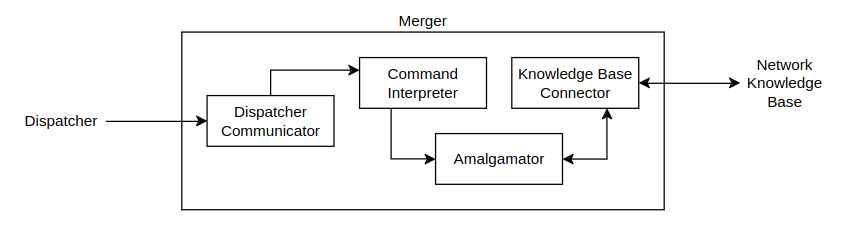
\includegraphics[width=14cm, height=8cm]{merger}
  \centering
\end{figure}

\FloatBarrier


\subsubsection{GUI} 
La GUI (Graphical User Interface) è un'interfaccia grafica che viene provvista a gli amministratori di rete per richiedere scansioni e visualizzarne i risultati.

\FloatBarrier

\chapter{Implementazione}

\section{Identificazione univoca dei probe}
Per distinguire i probe abbiamo deciso di utilizzare il loro indirizzo MAC (Medium Access Controll) ovvero un indirizzo di 12 caratteri alfanumerici (es. 00:11:22:33:44:55) che viene assegnato ad ogni dispositivo di rete e indentifica in modo univoco la scheda di rete del dispositivo.

\section{Parsing XML}
Lo scan di NMAP ritorna uno stream di dati in XML molto grande ed aspettare che l'intero stream di dati finisca per poi effettuare il parsing può essere pericoloso (es. va via la corrente e si perdono ore di computazione). Analizzando la struttura del XML che viene generato da NMAP tramite l'apposito DTD (Document Type Definition) abbiamo dedotto che fare un parsing incrementale su ogni tag host è la soluzione più ottimale per diminuire possibili problemi.

\section{Configurazione}
!TODO

\section{Software usati}

\subsection{Backbone di comunicazione}
Per comunicare con i probe situati per la rete viene usato MQTT (Message Queuing Telemtry Transport). 
MQTT è un protocollo di messaggistica leggero e public/subscribe progettato per l'Internet of Things (IoT).
Come broker MQTT viene usato Mosquitto per il suo supporto al Qualify of Service livello 2 che garantisce la recezione di messaggi exactly-once fra i probes e il sistema.

\subsection{Scanner}
I probe per eseguire le analisi usano NMAP che è una utility gratis ed open source per fare network discovery anche usata da moltissimi amministratori di reti per fare inventari di rete e monitorare host e servizi. 

\subsection{Database}
!TODO

\subsection{Tauri}
Tauri è un framework innovativo che permette di creare applicazioni desktop utilizzando tecnologie web familiari come HTML, CSS, JS. L'applicazione web, invece di venire eseguita in un browser, è trasformata in un'app desktop completa, con tutte le funzionalità native di un'applicazione tradizionale.
Per il frontend abbiamo scelto di usare principalmente React, e per il backend Rust.

\subsection{Rust}
Rust è un linguaggio di programmazione moderno, compliato e multi-paradigma, sviluppato da Mozilla Research in collaborazoine con la comunità open-source. Nato con l'obiettivo di coniugare efficienza, sicurezza e affidabilità, Rust si distingue per le sue caratteristiche peculiari:
\begin{itemize}
  \item \textbf{Sicurezza della memoria}: Rust elimina la possibilità di dangling pointers e memory leaks, tipici problemi di altri linguaggi che causano crash e comportamenti inaspettati.
  \item \textbf{Prestazioni elevate}: Rust offre prestazioni paragonabili a quelle del C++, grazie alla compilazione in codice macchina efficiente e all'assenza di runtime overhead.
  \item \textbf{Concorrenza sicura}: Rust gestisce la concorrenza in modo nativo, prevenendo automaticamente i data race e garantendo la sicurezza dei thread senza la necessità di complessi meccanismi di sincronizzazione.
  \item \textbf{Produttività}: Rust offre un sistema di ownership moderno e un potente sistema di tipi che aiutano a scrivere codice pulito, conciso e robusto.
\end{itemize}


\subsection{TypeScript}
TypeScript è un superset di JavaScript, ovvero un linguaggio che estende le sue funzionalità con tipi statici, classi, interfacce e moduli opzionali. È stato sviluppato da Microsoft e rilasciato nel 2012, guadagnando rapidamente popolarità nella community di sviluppo web.
Dei punti chiave di TypeScript sono:


\section{Frameworks e librerie}
\subsection{Rust}
Le librerie principali usate in Rust sono:
\begin{itemize}
  \item \textbf{Serde}: un framwork per la serializzazione e la deserializzazione per Rust, che consente di convertire facilmente dati strutturati in formati binari come JSON, BSON, XML ed altri. 
  \item \textbf{Tokio}: un runtime asincrono per Rust. Fornisce i mattoni essenziali per la scrittura di applicazioni di rete offrendo elevata velocità, scalabilità, facilità d'uso, affidabilità, robustezza e flessibilità.
  \item \textbf{Tracing} è uno strumento prezioso per la risoluzione dei problemi, il debug e il monitoraggio delle prestazioni di applicazioni Rust complesse.
\end{itemize}

\subsection{TypeScript}
La libreria principale per l'interfaccia grafica è React, una libreria open-source sviluppata da Meta per la creazoine di interfacce utente dinamiche e perfomanti. 
Permette di costruire UI complesse scomponendole in componenti riutilizzabili, facilidando lo sviluppo e la manutenzoine di applicazioni web.

\begin{itemize}
  \item \textbf{Tipizzazione statica}: TypeScript consente di definire i tipi di dati per variabili e funzioni, migliorando la leggibilità, la manutenibilità e la robustezza del codice. Il compilatore di TypeScript verifica che i tipi vengano utilizzati correttamente, aiutando a prevenire errori durante l'esecuzione.
  \item \textbf{Maggiori funzionalità}: TypeScript introduce concetti come classi, interfacce e moduli, che facilitano la scrittura di codice strutturato, modulare e scalabile. Queste funzionalità sono particolarmente utili per progetti di grandi dimensioni.
  \item \textbf{Compilazione in JavaScript}: Il codice TypeScript viene compilato in JavaScript puro, che può essere eseguito da qualsiasi browser o motore JavaScript. Questo significa che è possibile utilizzare TypeScript per sviluppare applicazioni web moderne senza preoccuparsi della compatibilità.
\end{itemize}


%% Capitolo
\chapter{Lavoro principale}
In hac habitasse platea dictumst. Vestibulum consectetur dictum pellentesque. Suspendisse nunc neque, commodo ac imperdiet nec, sollicitudin vitae libero. Donec bibendum vel nunc vitae pharetra. In vel volutpat odio, et interdum dui. Duis mauris ligula, congue eget molestie at, tincidunt nec diam. Nam vitae eros nec arcu suscipit vehicula. Aliquam consectetur imperdiet elit, eget pretium arcu fringilla at. Maecenas \cite{Knu86} sed libero pulvinar, mattis tortor vel, fermentum enim.


%% Capitolo
\chapter{Risultati}
In hac habitasse platea dictumst. Vestibulum consectetur dictum pellentesque. Suspendisse nunc neque, commodo ac imperdiet nec, sollicitudin vitae libero. Donec bibendum vel nunc vitae pharetra. In vel volutpat odio, et interdum dui. Duis mauris ligula, congue eget molestie at, tincidunt nec diam. Nam vitae eros nec arcu suscipit vehicula. Aliquam consectetur imperdiet elit, eget pretium arcu fringilla at. Maecenas \cite{Knu86} sed libero pulvinar, mattis tortor vel, fermentum enim.


%% Capitolo
\chapter{Conclusioni}
In hac habitasse platea dictumst. Vestibulum consectetur dictum pellentesque. Suspendisse nunc neque, commodo ac imperdiet nec, sollicitudin vitae libero. Donec bibendum vel nunc vitae pharetra. In vel volutpat odio, et interdum dui. Duis mauris ligula, congue eget molestie at, tincidunt nec diam. Nam vitae eros nec arcu suscipit vehicula. Aliquam consectetur imperdiet elit, eget pretium arcu fringilla at. Maecenas \cite{Knu86} sed libero pulvinar, mattis tortor vel, fermentum enim.

%% Fine dei capitoli normali, inizio dei capitoli-appendice (opzionali)
\appendix

%\part{Appendici}

\chapter{Titolo della prima appendice}
Sed purus libero, vestibulum ut nibh vitae, mollis ultricies augue. Pellentesque velit libero, tempor sed pulvinar non, fermentum eu leo. Duis posuere eleifend nulla eget sagittis. Nam laoreet accumsan rutrum. Interdum et malesuada fames ac ante ipsum primis in faucibus. Curabitur eget libero quis leo porttitor vehicula eget nec odio. Proin euismod interdum ligula non ultricies. Maecenas sit amet accumsan sapien.

%% Parte conclusiva del documento; tipicamente per riassunto, bibliografia e/o indice analitico.
\backmatter

%% Riassunto (opzionale)
%\summary
%Maecenas tempor elit sed arcu commodo, dapibus sagittis leo egestas. Praesent at ultrices urna. Integer et nibh in augue mollis facilisis sit amet eget magna. Fusce at porttitor sapien. Phasellus imperdiet, felis et molestie vulputate, mauris sapien tincidunt justo, in lacinia velit nisi nec ipsum. Duis elementum pharetra lorem, ut pellentesque nulla congue et. Sed eu venenatis tellus, pharetra cursus felis. Sed et luctus nunc. Aenean commodo, neque a aliquam bibendum, mauris augue fringilla justo, et scelerisque odio mi sit amet diam. Nulla at placerat nibh, nec rutrum urna. Donec ut egestas magna. Aliquam erat volutpat. Phasellus vestibulum justo sed purus mattis, vitae lacinia magna viverra. Nulla rutrum diam dui, vel semper mi mattis ac. Vestibulum ante ipsum primis in faucibus orci luctus et ultrices posuere cubilia Curae; Donec id vestibulum lectus, eget tristique est.

%% Bibliografia (praticamente obbligatoria)
\bibliographystyle{plain_\languagename}%% Carica l'omonimo file .bst, dove \languagename è la lingua attiva.
%% Nel caso in cui si usi un file .bib (consigliato)
\bibliography{thud}
%% Nel caso di bibliografia manuale, usare l'environment thebibliography.

%% Per l'indice analitico, usare il pacchetto makeidx (o analogo).

\end{document}

--- Istruzioni per l'aggiunta di nuove lingue ---
Per ogni nuova lingua utilizzata aggiungere nel preambolo il seguente spezzone:
    \addto\captionsitalian{%
        \def\abstractname{Sommario}%
        \def\acknowledgementsname{Ringraziamenti}%
        \def\authorcontactsname{Contatti dell'autore}%
        \def\candidatename{Candidato}%
        \def\chairname{Direttore}%
        \def\conclusionsname{Conclusioni}%
        \def\cosupervisorname{Co-relatore}%
        \def\cosupervisorsname{Co-relatori}%
        \def\cyclename{Ciclo}%
        \def\datename{Anno accademico}%
        \def\indexname{Indice analitico}%
        \def\institutecontactsname{Contatti dell'Istituto}%
        \def\introductionname{Introduzione}%
        \def\prefacename{Prefazione}%
        \def\reviewername{Controrelatore}%
        \def\reviewersname{Controrelatori}%
        %% Anno accademico
        \def\shortdatename{A.A.}%
        \def\summaryname{Riassunto}%
        \def\supervisorname{Relatore}%
        \def\supervisorsname{Relatori}%
        \def\thesisname{Tesi di \expandafter\ifcase\csname thud@target\endcsname Laurea\or Laurea Magistrale\or Dottorato\fi}%
        \def\tutorname{Tutor aziendale%
        \def\tutorsname{Tutor aziendali}%
    }
sostituendo a "italian" (nella 1a riga) il nome della lingua e traducendo le varie voci.
